\documentclass[tikz, border=10pt]{standalone}
\usetikzlibrary{positioning, arrows.meta, calc}

\begin{document}

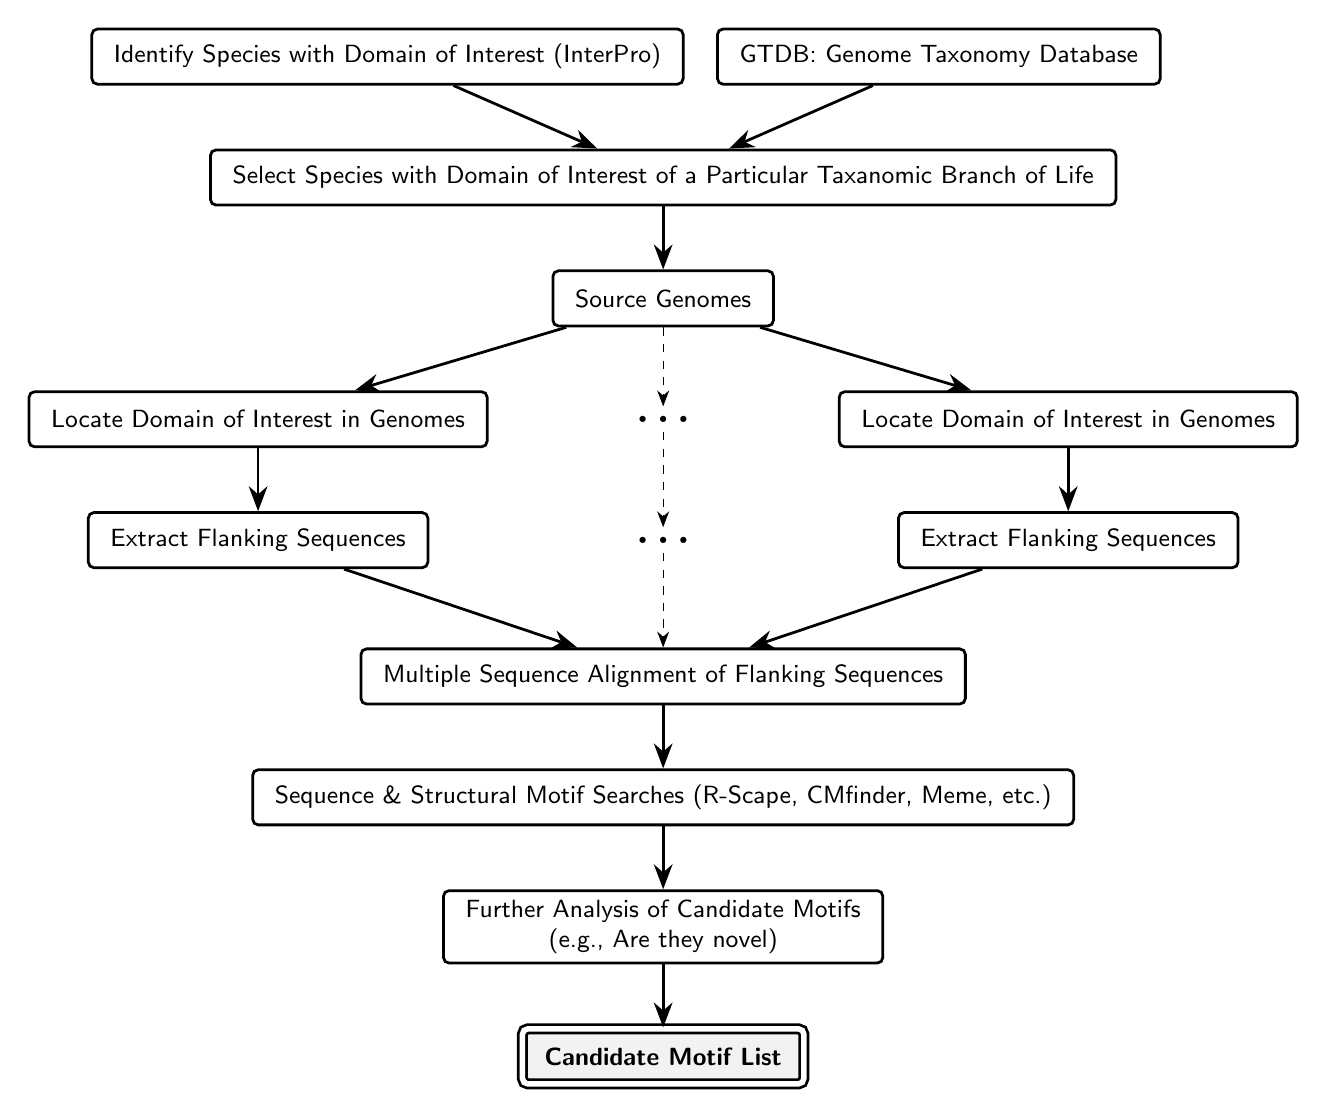
\begin{tikzpicture}[
    node distance=0.8cm and 0.4cm,
    % Base style for all steps
    step_node/.style={
        rectangle, 
        rounded corners=2pt, 
        draw=black, 
        line width=1pt, 
        font=\sffamily\small, 
        minimum height=0.7cm,
        inner xsep=8pt,
        align=center,
        fill=white
    },
    % Special style for the final result
    result_node/.style={
        step_node,
        double,            % Gives it a double border
        double distance=2pt,
        fill=gray!10,
        font=\sffamily\bfseries\small % Bold to show it's the end goal
    },
    dots/.style={
        font=\boldmath\Large,
        text=black
    },
    arrow/.style={
        -{Stealth[scale=1.2]}, 
        line width=1pt, 
        draw=black
    }
]

    % --- LEVEL 1: Data Sources ---
    \node[step_node] (interpro) {Identify Species with Domain of Interest (InterPro)};
    \node[step_node, right=of interpro] (gtdb) {GTDB: Genome Taxonomy Database};

    % --- LEVEL 2: Selection ---
    \node[step_node, below=of $(interpro.south)!0.5!(gtdb.south)$] (select) {Select Species with Domain of Interest of a Particular Taxanomic Branch of Life};

    % --- LEVEL 3: Genomes ---
    \node[step_node, below=of select] (download) {Source Genomes};

    % --- LEVEL 4: Domain Analysis (Parallel) ---
    \node[step_node, below left=0.8cm and 0.8cm of download] (locate1) {Locate Domain of Interest in Genomes};
    \node[step_node, below right=0.8cm and 0.8cm of download] (locateN) {Locate Domain of Interest in Genomes};
    \node[dots] (dots1) at ($(locate1)!0.5!(locateN)$) {$\dots$};

    % --- LEVEL 5: Flanking ---
    \node[step_node, below=of locate1] (flank1) {Extract Flanking Sequences};
    \node[step_node, below=of locateN] (flankN) {Extract Flanking Sequences};
    \node[dots] (dots2) at ($(flank1)!0.5!(flankN)$) {$\dots$};

    % --- LEVEL 6: MSA ---
    \node[step_node, below=1.2cm of dots2] (msa) {Multiple Sequence Alignment of Flanking Sequences};

    % --- LEVEL 7: Motif Searches ---
    \node[step_node, below=of msa] (motif) {Sequence \& Structural Motif Searches (R-Scape, CMfinder, Meme, etc.)};

    % --- LEVEL 8: Further Analysis ---
    \node[step_node, below=of motif] (further) {Further Analysis of Candidate Motifs \\ (e.g., Are they novel)};

    % --- LEVEL 9: FINAL OUTPUT ---
    \node[result_node, below=0.8cm of further] (final) {Candidate Motif List};

    % --- DRAW EDGES ---
    \draw[arrow] (interpro) -- (select);
    \draw[arrow] (gtdb) -- (select);
    \draw[arrow] (select) -- (download);
    
    \draw[arrow] (download) -- (locate1);
    \draw[arrow] (download) -- (locateN);
    \draw[arrow, dashed, thin] (download) -- (dots1);
    
    \draw[arrow] (locate1) -- (flank1);
    \draw[arrow] (locateN) -- (flankN);
    \draw[arrow, dashed, thin] (dots1) -- (dots2);
    
    \draw[arrow] (flank1) -- (msa);
    \draw[arrow] (flankN) -- (msa);
    \draw[arrow, dashed, thin] (dots2) -- (msa);

    \draw[arrow] (msa) -- (motif);
    \draw[arrow] (motif) -- (further);
    \draw[arrow] (further) -- (final);

\end{tikzpicture}

\end{document}
